\section{Results: the exclusion region}\label{sec:results}

\subsection{The 470-point physical grid}

Applying the likelihood of Eq.~\eqref{eq:lik} to the 470 points gives an expected limit that ranges from $\mu_{95}=0.00315$ at the heaviest mediator to the numerical cap of the scan, $\mu_{95}=64$, at the weakest coupling of the lightest one, a span of more than four orders of magnitude. The cap is a lower bound imposed by the likelihood scan and not a measured value. \textbf{381 points are excluded at 95\% CL and 89 survive, 43 of them in the $M_V=20$~GeV column.} Every point at or above 100~GeV is excluded. From 30 to 90~GeV the excluded region occupies the coupling range above $g_t\approx0.17$, except for the last few points of the 30 and 40~GeV columns, where the window closes (Table~\ref{tab:columns}). Only at 20~GeV is the column dominated by survivors, and there the single nominally excluded point sits at $g_t=0.249$ and lies within one standard deviation of unity once the Monte Carlo uncertainty of the template is propagated (Section~\ref{sec:sys}); no exclusion is established at 20~GeV.

The classification above is nominal: a point is excluded when $\mu_{95}<1$. Requiring $\mu_{95}+2\sigma_{\rm MC}<1$, with the Monte Carlo uncertainty of each template propagated as in Section~\ref{sec:sys}, turns this into a two-standard-deviation statement. The test was carried out for the 132 points at 20--40~GeV, where the selected yields are smallest; no such test was performed for the remaining 338 points. For those 132 the nominal 1, 34 and 36 exclusions at 20, 30 and 40~GeV become 0, 32 and 32, and the single point at 20~GeV, two at 30~GeV and four at 40~GeV sit within $2\sigma$ of the boundary. Points with $\mu_{95}<0.3$ are unaffected at the quoted precision. We therefore quote the nominal counts in Table~\ref{tab:columns} and give the robust subset separately.

Table~\ref{tab:columns} breaks the result down by mediator mass. The fraction of excluded points is 1/44 at 20~GeV, rises to 34/44 at 30~GeV and 36/44 at 40~GeV, stays at 37--38 of 44 through 50--80~GeV, and reaches unity at 100~GeV and above, while the smallest limit in each column falls from $1.6\times10^{-2}$ at 90~GeV to $3.2\times10^{-3}$ at 200~GeV. The excluded region is therefore not a wedge that closes with mass: it is bounded from below by a nearly horizontal line across the whole mass range, and its upper boundary survives only where the invisible width collapses inside the scanned coupling range.

\begin{table}[t]
\centering
\caption{Expected limits by mediator-mass column. The last two columns give the smallest and largest $\mu_{95}$ within the column; the entry $64$ marks the numerical cap of the likelihood scan and is a lower bound rather than a measured value. The surviving points are those with nominal $\mu_{95}>1$.}
\label{tab:columns}
\begin{tabular}{cccccc}
\toprule
$M_V$ [GeV] & points & excluded & surviving & largest surviving $g_t$ & $\mu_{95}$ range \\
\midrule
 20 & 44 & 1 & 43 & 3.5449 & 0.938--64 \\
 30 & 44 & 34 & 10 & 3.5449 & 0.099--2.93 \\
 40 & 44 & 36 & 8 & 3.5449 & 0.105--3.21 \\
 50 & 44 & 37 & 7 & 0.1645 & 0.085--2.58 \\
 60 & 44 & 38 & 6 & 0.1514 & 0.055--3.11 \\
 70 & 44 & 37 & 7 & 0.1645 & 0.031--2.67 \\
 80 & 43 & 37 & 6 & 0.1650 & 0.023--2.70 \\
 90 & 38 & 36 & 2 & 0.1790 & 0.017--1.05 \\
100 & 34 & 34 & 0 & --- & 0.011--0.61 \\
120 & 27 & 27 & 0 & --- & 0.007--0.20 \\
140 & 22 & 22 & 0 & --- & 0.005--0.10 \\
160 & 17 & 17 & 0 & --- & 0.003--0.04 \\
180 & 14 & 14 & 0 & --- & 0.004--0.03 \\
200 & 11 & 11 & 0 & --- & 0.003--0.02 \\
\bottomrule
\end{tabular}
\end{table}

\subsection{The exclusion boundary}

Figure~\ref{fig:map} is the main result of the paper. Every coloured rectangle is one computed point: the cell spans the logarithmic midpoints between neighbouring $g_t$ values of the same column and the midpoints between neighbouring $M_V$ columns, so no colour is interpolated in either direction and nothing is drawn outside the computed range of a column. The colour encodes $\mu_{95}$ at the central abundance solution and the cells are the points at which the likelihood was evaluated. Of the $14\times44=616$ coordinates in the frame, 470 are computed, 51 have no root of the abundance equation at the fixed mass splitting $\Delta m=1$~MeV used in the recoil normalisation, and 95 have a root but violate $\Gamma_V/M_V<3\%$, where the narrow-width treatment does not apply (58 of these also fail $M_V-2m_\chi\ge5\Gamma_V$). All 146 grey cells lie at $M_V\ge80$~GeV with $g_t\le1.42$; neither kind is an allowed region, and every coordinate inside the frame has been evaluated.

\begin{figure}[t]
\centering
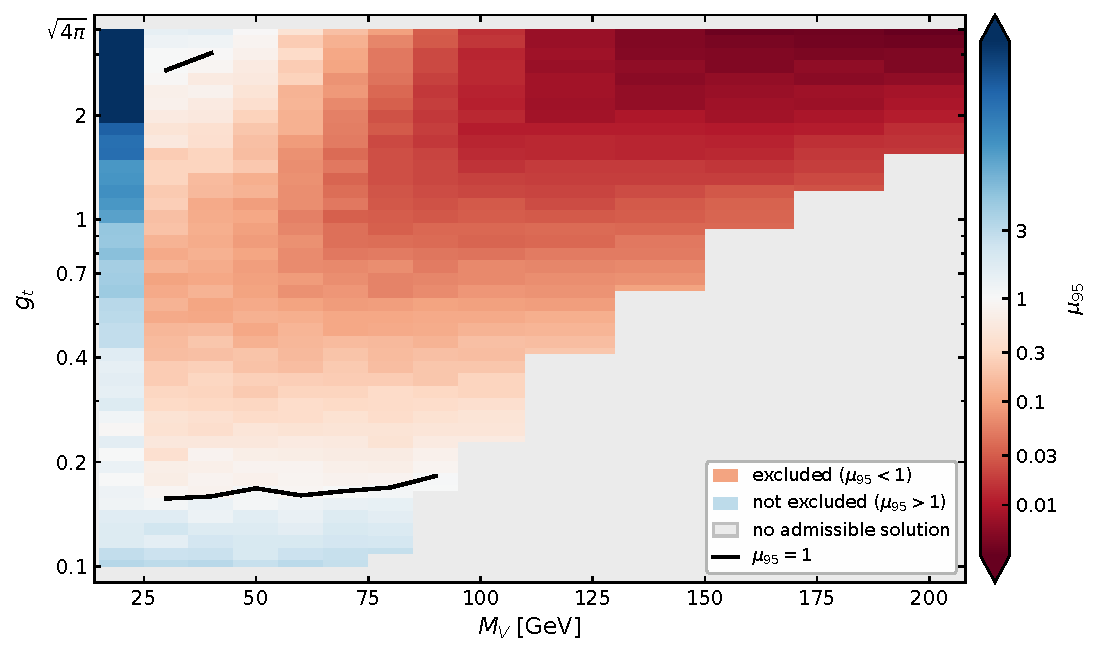
\includegraphics[width=0.88\textwidth]{figs/fig2_v10.pdf}
\caption{Expected CMS $t\bar t$+MET 95\% CL limits on the branch satisfying the recoil-yield, central-abundance and narrow-width conditions, at $\sqrt{s}=13$~TeV with $138\ \mathrm{fb}^{-1}$. Each cell is one computed grid point and no colour is interpolated; red is $\mu_{95}<1$, blue $\mu_{95}>1$, and the neutral tone marks unity. The black line joins the nominal $\mu_{95}=1$ crossings of adjacent columns and is interrupted where the crossing moves by more than a factor 1.5 between them. Grey cells have no admissible solution; circles mark cells at the scan cap, $\mu_{95}=64$.}
\label{fig:map}
\end{figure}

The boundary has two pieces. A lower envelope, nearly flat at $g_t\approx0.15$--$0.19$, runs from 30 to about 90~GeV and separates the production-limited region beneath it; the 20~GeV column has its boundary at $g_t\approx0.24$ with a single point above it; above 100~GeV even the smallest admissible coupling is excluded, so the envelope ends there. An upper edge appears only where the invisible branching ratio falls steeply inside the scanned range: at $g_t\approx2.7$ and $3.0$ for 30 and 40~GeV the window closes and the last computed points return above unity, while from 50 to 90~GeV no such collapse occurs inside $g_t\le\sqrt{4\pi}$ and the excluded region extends to the top of each column. At 20~GeV a single point near $g_t\approx0.25$ is nominally excluded but lies within the Monte Carlo uncertainty of the boundary, so it is not a resolved edge. The closure would move by more than a factor of ten between the 20 and 30~GeV columns with no computed point between them, and no line is drawn across that interval. The points closest to the lower boundary are 1008 ($\mu_{95}=1.000$), 227 ($1.010$) and 2061 ($1.010$), the smallest distance to unity being $0.03\%$, far below the systematic band of Section~\ref{sec:sys}.


\subsection{The two coupling regimes}

Figure~\ref{fig:curves} shows the expected limit as a function of $g_t$ for several mediator masses. Over most of the scanned range the limit falls steeply: the cross section grows roughly as $g_t^2$, so each step in coupling gives a proportionally larger signal. The fall flattens at large $g_t$ and, in the heavier columns, reverses. At $M_V=100$~GeV, the column with the clearest turnover among those shown in Fig.~\ref{fig:curves}, the limit flattens at $\mu_{95}\approx0.013$ between $g_t=2.5$ and $3.3$ and then rises to $0.016$ at $g_t=3.55$, by which point the invisible branching ratio has fallen to $0.14$. The mediator is increasingly decaying into quarks, and the fraction of its decays that produces missing momentum shrinks accordingly.

The same competition is visible more sharply at low mass: at $M_V=30$~GeV the excluded window runs from $g_t\approx0.16$ to $2.7$, with the limit falling from $1.0$ at the lower edge to $0.10$ at its minimum and rising again to $1.45$ at the largest scanned coupling. The turnover is decisive only below 50~GeV: at 30 and 40~GeV it closes the window at $g_t\approx2.7$ and $3.0$. From 50 to 90~GeV the same competition never brings the limit back above unity anywhere inside $g_t\le\sqrt{4\pi}$, so the excluded band continues to the largest admissible coupling, and the top of the coloured region in Fig.~\ref{fig:map} is the upper end of the scanned coupling range, $g_t=\sqrt{4\pi}$, rather than a boundary of the model. The invisibility penalty is visible as a flattening and a partial recovery of the limit; it closes the window only at 30 and 40~GeV, where the recovery reaches unity.

\begin{figure}[htbp]
\centering
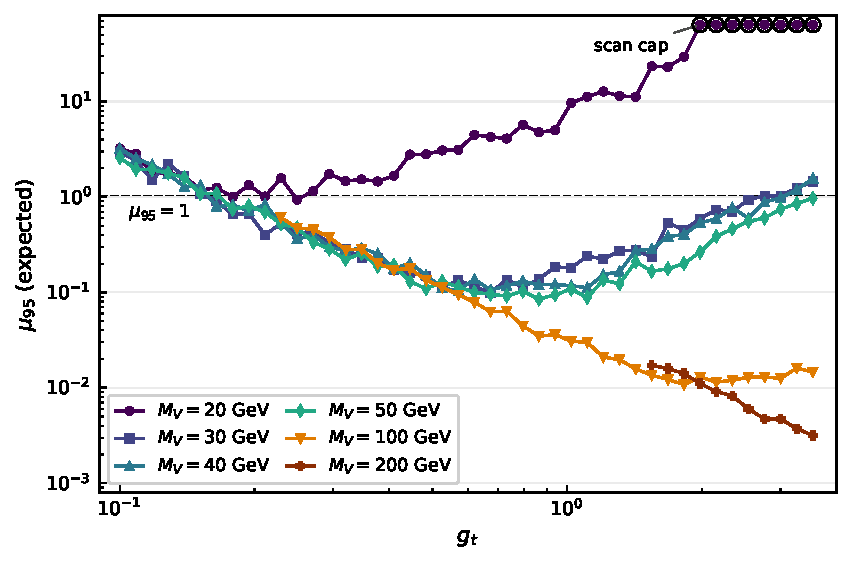
\includegraphics[width=0.84\textwidth]{figs/fig3_v10.pdf}
\caption{Expected limit $\mu_{95}$ as a function of $g_t$ for six mediator masses. The dashed line is $\mu_{95}=1$. The 30 and 40~GeV curves fall below unity, turn over and return above it at $g_t\approx2.7$ and $3.0$, closing the excluded window; from 50~GeV upward the recovery does not reach unity inside $g_t\le\sqrt{4\pi}$; at 20~GeV the limit fluctuates about unity and the exclusion is not resolved. Open circles mark points at the numerical cap, $\mu_{95}=64$.}
\label{fig:curves}
\end{figure}

Whether the turnover actually reopens the window is decided by the absolute level of the signal at the largest coupling, not by the size of the drop. The yield is $N_{\rm SR}=138000\,\varepsilon\,\sigma_{\rm vis}$, and $\varepsilon$ itself grows with $M_V$ (Table~\ref{tab:eff}): the same cross section therefore gives a larger signal in a heavier column. Figure~\ref{fig:vis} shows the two ingredients. At $M_V=20$~GeV the visible cross section falls by a factor 111 between its peak and $g_t=\sqrt{4\pi}$, and the column reopens at $g_t\approx0.25$. At 30 and 40~GeV it falls by a factor of 13 and 15 and the last points land at $\sigma_{\rm vis}\approx0.13$ and $0.10$~pb, where the yield falls below the level the likelihood excludes at 95\% CL and the expected limit returns above unity. At 50~GeV the drop is of the same order, 11, but the efficiency is twice as large as at 30~GeV, so the same cross section produces twice the signal and the column stays excluded all the way to $\sqrt{4\pi}$. The exclusion is set by the signal yield, its fifteen-bin shape and the likelihood, not by the cross section alone; the cross-section level quotes where the turnover lands relative to that combination. The upper boundary is thus a property of $\varepsilon\sigma_{\rm vis}$, not of $\mathrm{BR_{inv}}$ alone.

\begin{figure}[htbp]
\centering
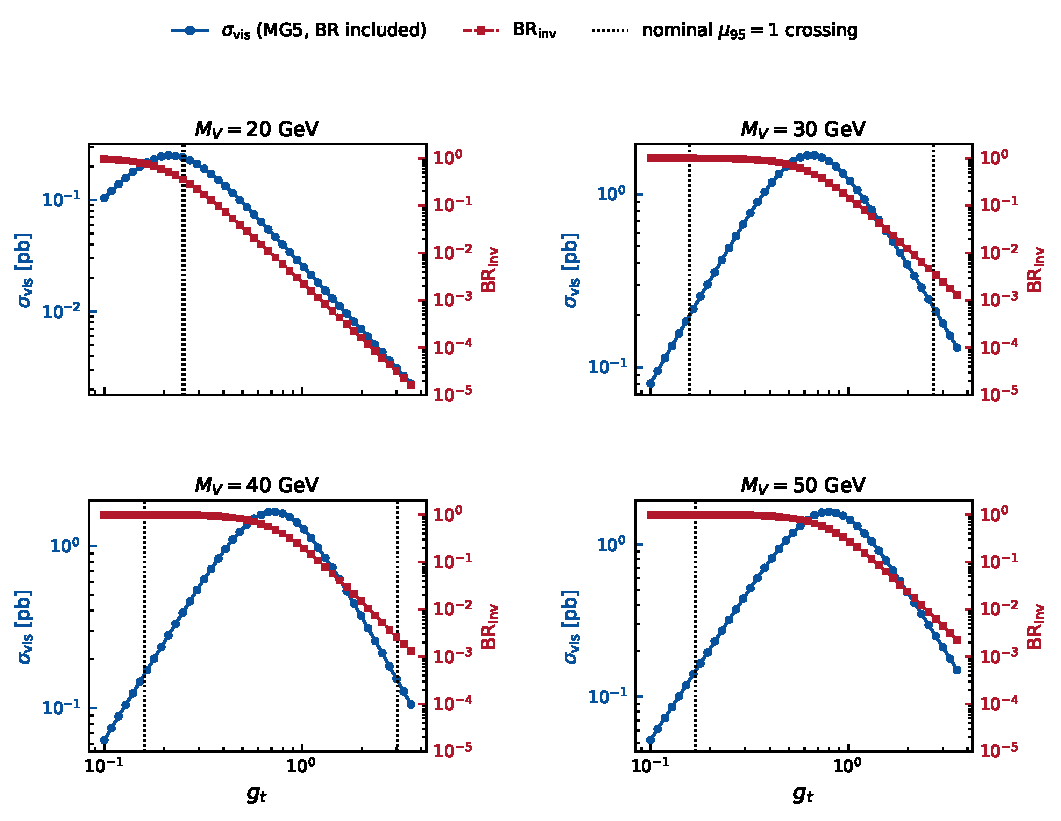
\includegraphics[width=0.97\textwidth]{figs/fig4_v10.pdf}
\caption{Visible cross section $\sigma_{\rm vis}$ (blue, left axis; MadGraph at leading order with the invisible decay of the mediator already included) and invisible branching ratio $\mathrm{BR_{inv}}$ (red, right axis) as a function of $g_t$, for four mediator masses. Dotted vertical lines mark the nominal $\mu_{95}=1$ crossings of each column. The cross section turns over in every column as $\mathrm{BR_{inv}}$ falls; whether the column reopens depends on where the turnover lands relative to the exclusion threshold, that is on $\varepsilon(M_V)\,\sigma_{\rm vis}$, not on the depth of the drop alone.}
\label{fig:vis}
\end{figure}

\FloatBarrier
